\documentclass[11pt]{article}
\usepackage[a4paper, margin=1in]{geometry}
\usepackage{tikz}
\usepackage{amsmath}
\usepackage{lmodern}
\usepackage{bm}
\usepackage{fancyhdr}
\usepackage{amsfonts}
\usepackage{amssymb}

\title{\textbf{CITS2211 Assignment 2}}
\author{Name: Baasil Siddiqui \\ Student Id: 23895849}
\date{}

\pagestyle{fancy}
\fancyhf{}

\fancyfoot[R]{Page \thepage\ of \pageref{LastPage}}

\begin{document}
\parskip 2mm
\maketitle
\thispagestyle{empty}

\section*{Question 1}
\subsection*{a)}
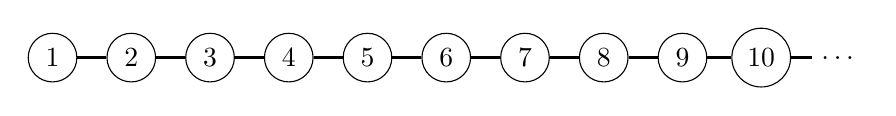
\begin{tikzpicture}
    \node[draw, circle] (top) at (0,0) {$1$};
    \node[draw, circle] [right of=top] (right) {$2$};
    \node[draw, circle] [right of=right] (rtr) {$3$};
    \node[draw, circle] [right of=rtr] (rtrr) {$4$};
    \node[draw, circle] [right of=rtrr] (rtrrr) {$5$};
    \node[draw, circle] [right of=rtrrr] (bottom) {$6$};
    \node[draw, circle] [right of=bottom] (bottom2) {$7$};
    \node[draw, circle] [right of=bottom2] (bottom3) {$8$};
    \node[draw, circle] [right of=bottom3] (bottom4) {$9$};
    \node[draw, circle] [right of=bottom4] (bottom5) {$10$};
    \node [right of=bottom5] (dots) {$\dots$};
    \draw[thick] (top) -- (right) -- (rtr) -- (rtrr) -- (rtrrr) --
          (bottom) -- (bottom2) -- (bottom3) -- (bottom4) --
          (bottom5) -- (dots);
\end{tikzpicture}

\subsection*{b)}

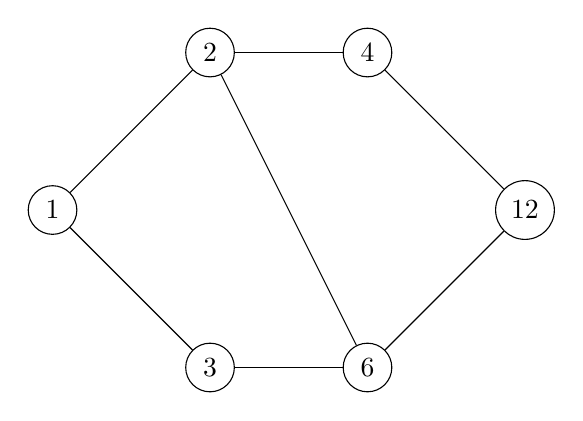
\begin{tikzpicture}
    \node[draw, circle] (one) at (0,0) {$1$};
    \node[draw, circle] (two) at (2,2) {$2$};
    \node[draw, circle] (three) at (2,-2) {$3$};
    \node[draw, circle] (four) at (4,2) {$4$};
    \node[draw, circle] (six) at (4,-2) {$6$};
    \node[draw, circle] (twelve) at (6,0) {$12$};

    \draw (one) -- (two);
    \draw (one) -- (three);
    \draw (two) -- (four);
    \draw (two) -- (six);
    \draw (three) -- (six);
    \draw (four) -- (twelve);
    \draw (six) -- (twelve);
\end{tikzpicture}

\end{document}

